\documentclass[11pt]{article}
\usepackage[utf8]{inputenc} % Para caracteres en espa�ol
\usepackage{amsmath,amsthm,amsfonts,amssymb,amscd}
\usepackage{multirow,booktabs}
\usepackage[table]{xcolor}
\usepackage{fullpage}
\usepackage{lastpage}
\usepackage{enumitem}
\usepackage{multicol}
\usepackage{fancyhdr}
\usepackage{mathrsfs}
\usepackage{wrapfig}
\usepackage{setspace}
\usepackage{esvect}
\usepackage{calc}
\usepackage{multicol}
\usepackage{cancel}
\usepackage{graphicx}
\graphicspath{ {pictures/} }
\usepackage[retainorgcmds]{IEEEtrantools}
\usepackage[margin=3cm]{geometry}
\usepackage{amsmath}
\newlength{\tabcont}
\setlength{\parindent}{0.0in}
\setlength{\parskip}{0.05in}
\usepackage{empheq}
\usepackage{framed}
\usepackage{newtxmath}
\usepackage{euscript}
\DeclareMathAlphabet{\mathpzc}{T1}{pzc}{m}{it}
\usepackage[most]{tcolorbox}
\usepackage{xcolor}
\colorlet{shadecolor}{orange!15}
\parindent 0in
\parskip 12pt
\geometry{margin=1in, headsep=0.25in}
\theoremstyle{definition}
\newtheorem{defn}{Definition}
\newtheorem{reg}{Rule}
\newtheorem{exer}{Exercise}
\newtheorem{note}{Note}
\newcommand{\volume}{{\ooalign{\hfil$V$\hfil\cr\kern0.08em--\hfil\cr}}}
\newcommand{\parr}{\mathbin{\|}} % Parralel Symbol
\begin{document}
\setcounter{section}{2} %Section before the section you want. I want section 1 I put 0
\setcounter{page}{20} %page number you want to be the first page
\setcounter{equation}{17} %equation before the equation you want I want equation 2 I put 1
%\definecolor{babyblue}{rgb}{0.54, 0.81, 0.94}
\definecolor{babyblueeyes}{rgb}{0.63, 0.79, 0.95}
\definecolor{babyblue}{rgb}{0.69, 0.88, 0.9}

 \pagestyle{fancy}
 
\fancyhf{}
\rhead{Section 5:  Collisions}
\rfoot{Page \thepage}
\thispagestyle{empty}


\begin{center}
{\LARGE \bf Section 5:  Collisions}\\
{\large AE435}\\
Spring 2018
\end{center}

\vspace{5mm}
\section{Electron-Ion Collisions (Coulomb Collisions)}

Electron-Ion Collisions are very different from electron-atom collisions. %electron atoms, we think of atom just as billard ball model. Electron would have to get very close inorder to interact. 

%couloumb collisions are a long range collision.  
Coulomb collisions are a long range collision. Long-range forces are one characteristic distinguishing plasmas from neutral gases.  Since electromagnetic interactions have a much longer reach than atomic interactions, electron-ion cross-sections tend to be much larger than electron-neutral cross-sections.   As a corollary, the electron-ion collision frequency exceeds electron-neutral collision frequency, when the ionization fraction is above a few tenths of a percent. 

As a result we have to redefine what a collision is because they have a coulomb force acting on them. Collisions are happening continuously because the charges are always interacting.

 \begin{equation}
 \begin{aligned}
 \nu_{ei} > > \nu_{en}
 \end{aligned}
 \end{equation}
\vspace{5mm}
\tableofcontents
\newpage
\subsection{Elastic}
The long-range "collision" process between electrons-ions is really a continuous process:
 %here we are looking at electron moving thorugh sea of + ions. Trajectory continuously being changed becasue of these couloumb forces. As a result...
 \begin{center}
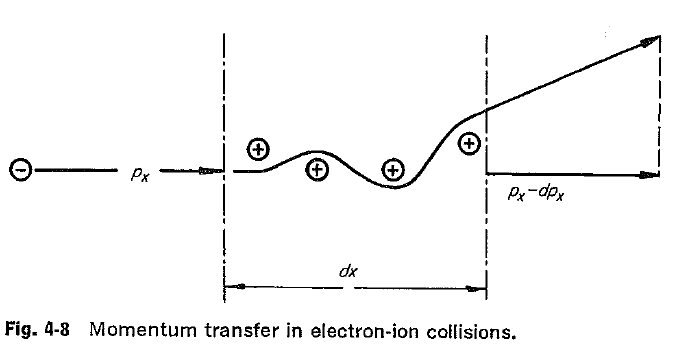
\includegraphics[scale=.9]{11.png}
\end{center}
 
Define the momentum transfer cross section            $Q_{ei}^{(P)}$      , where the $\hat{x}$-momentum, $P_x$,     	varies as
 \begin{equation}
 \begin{aligned}
\frac{\mathrm{d} P_x}{P_x} = n_+ \, Q_{ei}^{(P)} \, \mathrm{d} x
 \end{aligned}
 \end{equation}
 
Then we can define:%we can show that the collision cross section is .....
  %
  \begin{shaded}
  \textbf{Collision Cross Section}
  \begin{equation}
 \begin{aligned}
Q_{ei}^{(P)} = \frac{4 \, q_e^4}{(4\,\pi\,\varepsilon_o)^2\varepsilon^2} \, \ln\frac{8 \, \pi \, \varepsilon_o \, r_o \, \varepsilon}{q_e^2}
 \end{aligned}
 \end{equation}
Where
  \begin{equation*}
 \begin{aligned}
\varepsilon &= \text{Relative KE Before the Collision} \\
r_o &= \text{An Empirical Cutoff Distance for the Effective Range of the Coulomb Force}
 \end{aligned}
 \end{equation*}
 \end{shaded}
Best choice for the shielding distance of the plasma, $r_o$, works out to be the Debye Length, $\lambda_D$:
 
  \begin{equation}
 \begin{aligned}
 r_o = \lambda_D = \Bigg(\frac{\varepsilon_o \, k \, T_e}{n_e \, q_e^2}\Bigg)^{\frac{1}{2}}
 \end{aligned}
 \end{equation}
 
Combine logarithmic terms into the Coulomb Logarithm:
 
  \begin{equation}
 \begin{aligned}
 \ln \Lambda = \ln \frac{8 \, \pi \, \varepsilon_o \, r_o \, \varepsilon}{q_e^2}
 \end{aligned}
 \end{equation}
 
 Use the conversion of Energy into Temperature using:
  \begin{equation}
 \begin{aligned}
 \varepsilon = \frac{3}{2} \, k \, T_e
 \end{aligned}
 \end{equation}
 
For a broad range of typical plasma parameters, we can simplify:
  \begin{equation*}
 \begin{aligned}
 \ln \Lambda \approx 10
 \end{aligned}
 \end{equation*}
 This is an acceptable approximation for a broad range of typical plasma parameters. Even from a wide range of temperatures and densities (over orders of magnitude).
 
So the approximate momentum-transfer cross section is:
 \begin{shaded}
 \textbf{Approximate Momentum-Transfer Cross Section}
  \begin{equation}
 \begin{aligned}
 Q_{ei}^{(P)} \approx \frac{Q_o}{\varepsilon^2}
 \end{aligned}
 \end{equation}
 Where
  \begin{equation*}
 \begin{aligned}
 Q_o &= 6.5 \times 10^{-17} \qquad [m^2 \ eV^2]
 \end{aligned}
 \end{equation*}
 \end{shaded}
 
\textbf{Question: }How can we calculate collision frequency, $\nu_{ei}$?

\textbf{Answer: }Equations 15 or 14 in simplified form. We could have $ \nu_{ei} \approx n_e \, Q_{ei}^{(P)} \, \bar{v}_e$. This is only an approximation though because technically we should do the integration since they are both dependent on energy. But this is a good approximations nonetheless. 
\newpage
\subsection{Inelastic}
It's similar to an electron-atom collision because the electron has to penetrate into the ion core to remove another electron.

These are basically like electron-atom collisions. Doubly ionization as a result... 


\subsection{Radiation}
Charged particles deflected by Coulomb forces can radiate energy away as photons (bremsstrahlung).

It is possible for charged particles to be deflected (bent as it goes around ion) it can release radiation. However, in fusion plasma, this is important to consider since temperatures are very high. Electric propulsion plasmas never really get that hot, (usually 10-20eV) rarely hot enough for radiative collisions to be important enough to consider.

But the energies/temperatures in EP plasmas are rarely high enough for this to be important.

\end{document}